\section{Additional navigation model using occurrence variables (bag navigation)}

% Let $Occ = \{occ_1,...,occ_z\}$ be the variables encoding the evaluation of \inlineocl{src}, with $dom(occ_i)=\{0..|o|\}$. 

% To link $Y$ with $M$ and $Occ$, we define the navigation constraint:
% \begin{equation*}\label{csp:nav_def} 
% nav(Occ,T,Y) \iff
% \begin{aligned}
% \forall i \in [1,z],\forall j \in [1,p] : y_{(i-1)p+j} = T_{ptr_i \times p+j} \\
% \end{aligned}
% \end{equation*}

In this model $M$ is the adjacency matrix we're using to navigate.
There are $r$ rows and $c$ columns in $M$.
This model can be seen as adding a \textit{virtual row} $Occ'$ to $M$.
There are $c$ variables in $Occ'$.
The source expression variables $Occ$, can be a row or a \textit{virtual row} of a previous matrix $M'$, or $M$ in the case of a reflexive reference.
There are $r$ variables in $Occ$.
If the relation is reflexive, $r=c$.

Each variable in the new \textit{virtual row}, sums the column it corresponds to, for which each variable is multiplied by the corresponding variable from $Occ$. 
\begin{equation}\label{csp:nav}
nav(Occ,M,Occ'):
\begin{cases}
\forall j \in [1,c] :\\
    Occ_j' = sum([Occ_i*M_ij | i \in [1,r]])
\end{cases}
\end{equation}

\begin{figure}[!ht]
    \centering
    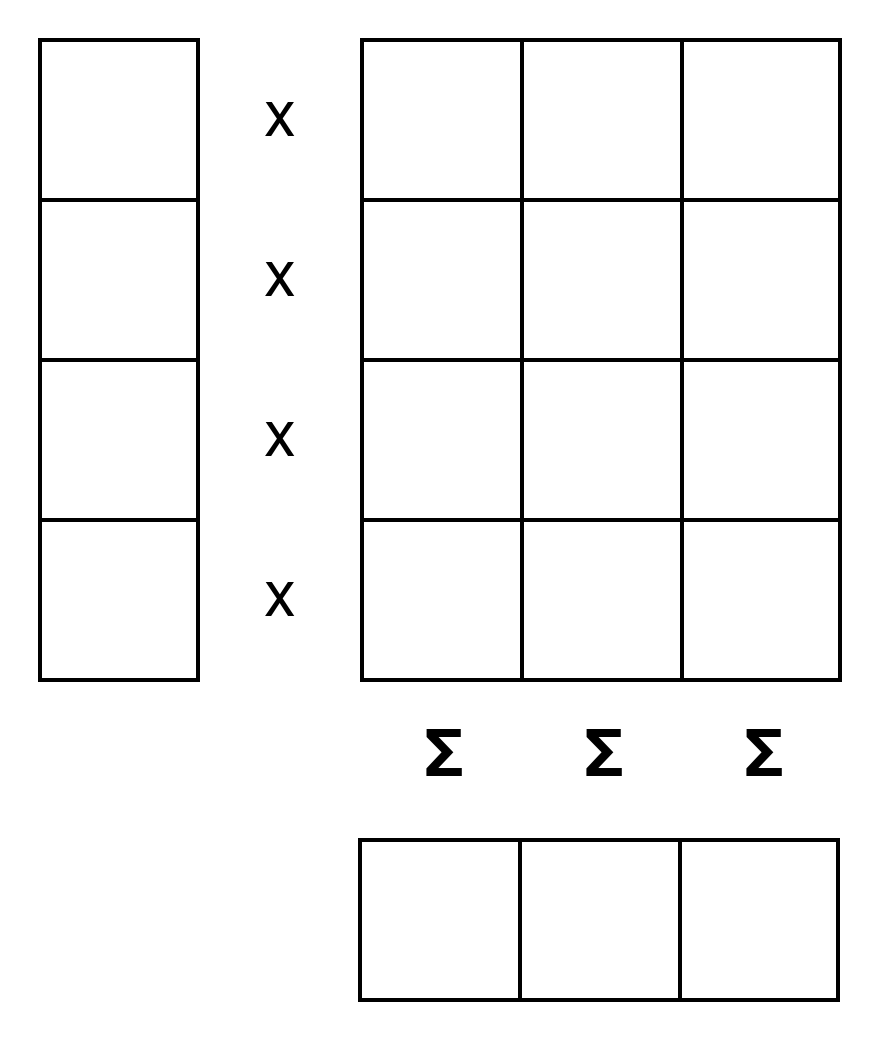
\includegraphics[trim={0 0 0 0},width=0.3\linewidth]{Contributions/OCLCSP/figures/navCSPOcc.png}
    \caption{Diagram of \textit{bag} navigation}
    % \label{fig:metamodel}
\end{figure}
In this diagram illustrates how the variables and constraints are organized spatially.
The incoming array $Occ$ is vertical to the left, the output array $Occ'$ is horizontal at the bottom.
We can see how each variable of $Occ$ multiplies a row of $M$, and each variable in $Occ'$ sums the column.

This additional model can be tied to the base model using $gcc$ in the same way as described in the UML CSP section.
However it can entirely replace the base model, when order doesn't matter, which can be detected by the interpretation process.

\subsection{Closure}
We will also use the adjacency matrix to model closure on a reflexive relation.
We can get trivially get a 0/1 matrix from the adjacency matrix preserving multiplicity.
Because the relation is reflexive, the adjacency matrix is square, of side size $z$
\begin{equation}\label{csp:nav}
    closure(X,M,Y):
    \begin{cases}
    \forall j \in [1,z] :\\
        Y_j = \bigvee([(X_i \wedge M_ij) \vee (Y_i \wedge M_ij) | i \in [1,z]])
    \end{cases}
\end{equation}
This model uses both the input and output to activate the column for the output variables.

\begin{figure}[!ht]
    \centering
    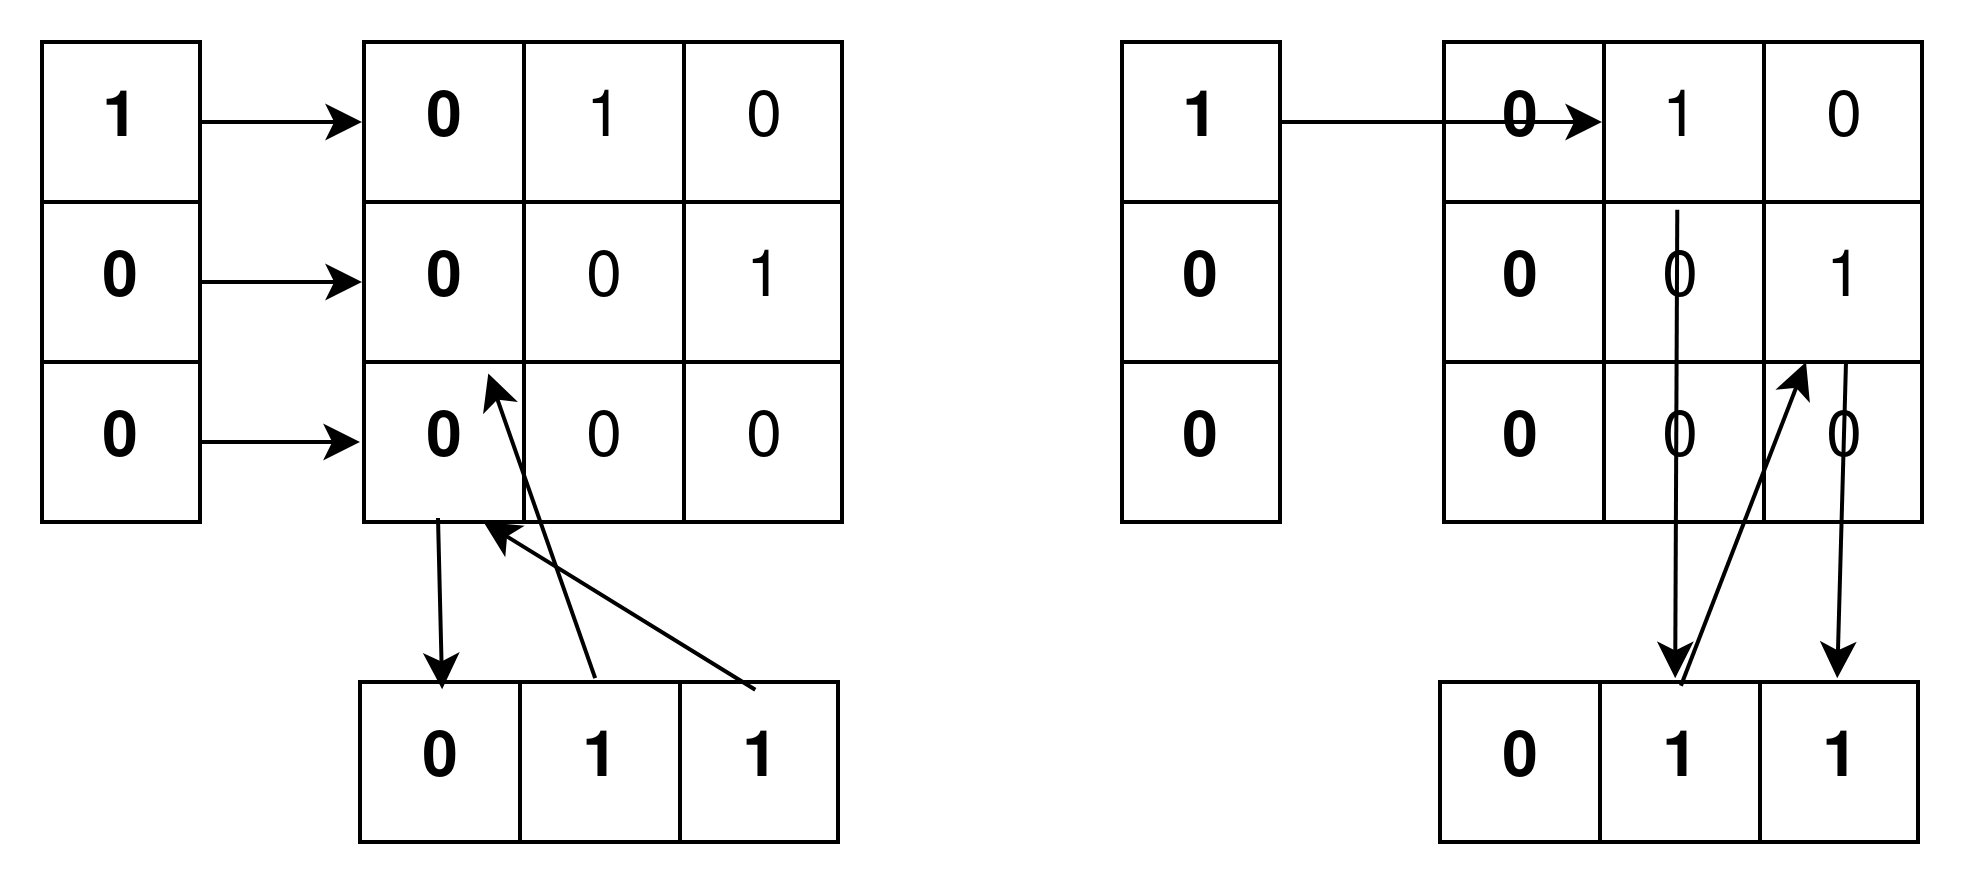
\includegraphics[trim={0 0 0 0},width=0.6\linewidth]{Contributions/OCLCSP/figures/navCSPclosure.png}
    \caption{Diagram of closure solution}
    % \label{fig:metamodel}
\end{figure}
In this figure the arrows towards the matrix are the \textit{and} between the values of the column and the input or output, and the arrow towards the output is the \textit{or} on the column.
In this diagram we see an expression equivalent to \inlineocl{self.ref.closure()} where \inlineocl{self} points to the first object, and \inlineocl{ref} is a reflexive reference.
The source occurrences point to the first object, but no relation in the \inlineocl{refTable} goes towards the first object. Hence, the first object isn't in the output.
However the first object points to the second, and having the second in the output gets us the third in the output.